\section{Code an Algorithm Inefficiencies}
\label{identification}

Inefficiency removal is a two stage iterative process. First, the application is analysed to identify the critical sections of the code that take the most time to compute. This can process can be automatised by using third party tools, such as GPROF, Callgrind, or VTune, which produce reports listing the percentage of time spent in each of the application functions. A more detailed analysis can be obtained using tools similar to PAPI, where hardware counters are measured to obtain cache miss rates, float point instructions, and other low level information.

The test environment used in both this section and section \ref{removal} is a dual-socket system with two Intel E5-2670v2 with 10 cores (20 hardware threads) at 2.5 GHz each, 256 KB L2 cache per core and 25 MB shared L3 cache, coupled with 64 GB DDR3 RAM. The KBest policy was adopted to ensure that the only the best, but consistent, time measurements are considered. A 5\% interval was used for a \textit{k} of 4, with a minimum of 12 and maximum of 24 time measurements.

In a preliminary analysis using Callgrind, the \ttDilepKinFit was identified as the most time consuming function, specially when considering a significant number of variations. Figure \ref{fig:ttDilepKinFit} shows the relative execution time for the \ttDilepKinFit, I/O of event loading, and the rest of the computations (the remaining cuts). \tth execution with 1024 variations was considered for all efficiency measurements, as it is a reasonable amount without an exaggerated compromise of the application execution time. Note that the application is dependant on the ROOT framework and LipMiniAnalysis library, which code cannot be modified.

\begin{figure}[!htp]
	\begin{center}
		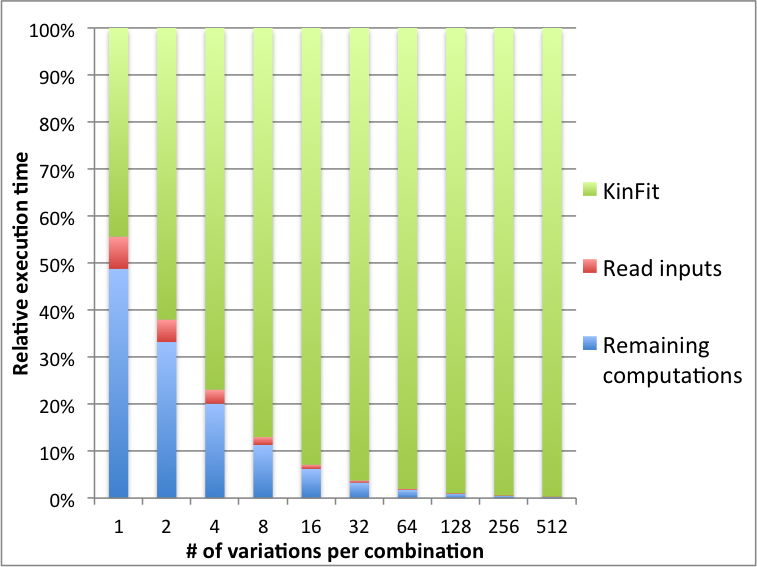
\includegraphics[scale=0.4]{charts/relative_exec_time_kinfit_rest.png}
		\caption{Relative execution time of the critical sections of the \tth application.}
		\label{fig:ttDilepKinFit}
	\end{center}
\end{figure}

A preliminary computational analysis determined that the application is compute bound on the test system, where accesses to the system RAM memory are not a limiting factor with a ratio of 8 instructions per byte fetched for 512 variations.

\subsection{Pseudo-Random Number Generation Inefficiencies}

Pseudo-random number generators (PRNGs) are common in many Monte Carlo simulation and reconstruction applications. A good PRNG deterministically generates uniform numbers with a long period, its values produced pass a set of randomness tests, and, in HPC, it must be efficient and scalable. Repeatability is ensured by providing a seed to the PRNG prior to number generation, due to their deterministic execution.

The variation for the kinematical and Higgs reconstructions is based on applying a random offset to the current particles characteristics. This offset has a maximum magnitude of 2\% of the original value and is determined by a PRNG. An analysis of the callgraph produced for 256 variations (higher variations made the Callgrind execution time infeasible) revealed that 63\% of \tth execution time was spent on the PRNG. However, 23\% of the time was spent on setting the seed for the PRNG. Figure \ref{fig:prng256} presents the callgraph for the \ttDilepKinFit function of \tth.

\begin{figure}[!htp]
	\begin{center}
		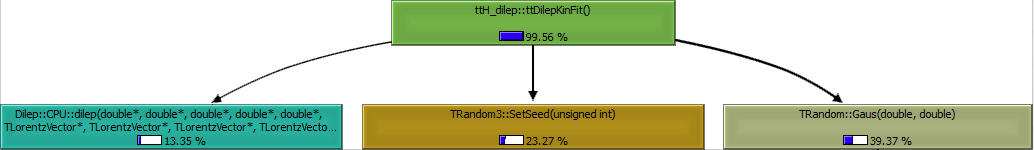
\includegraphics[scale=0.33]{images/prng_256.png}
		\caption{Callgraph subset of the \ttDilepKinFit most time consuming sections for 256 variations per combination.}
		\label{fig:prng256}
	\end{center}
\end{figure}

An analysis of the code revealed that the application uses a PRNG available in ROOT, which uses the Mersenne Twister algorithm, resetting the seed in every variation. The Mersenne Twister period is approximately $4.3 * 10^{6001}$, while the maximum amount of pseudo random numbers generated by the application, for the input file used and 512 variations, is $1.5 * 10^9$, making the seed reset unnecessary. The removal of this inefficiency granted an increase of 71\% in performance for 1024 variations.

%\begin{figure}[!htp]
%	\begin{center}
%		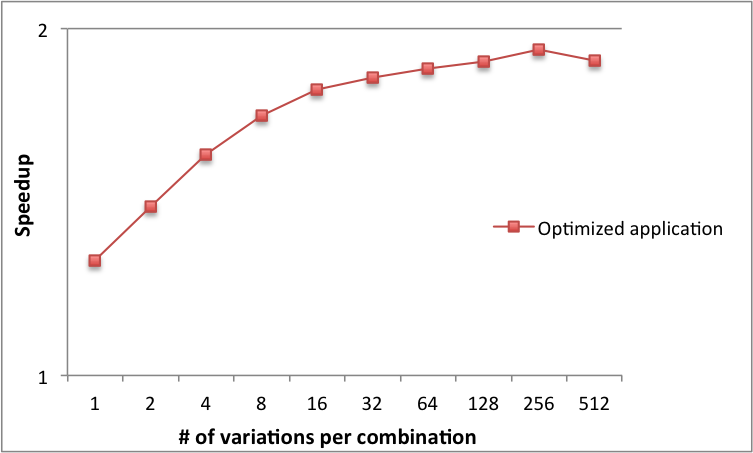
\includegraphics[scale=0.4]{charts/speedup_trandom_optim.png}
%		\caption{Schematic representation for the \tth application flow.}
%		\label{fig:PRNG}
%	\end{center}
%\end{figure}

\subsection{Data Structure Inefficiencies}

Even with the PRNG optimization the \ttDilepKinFit remains the critical region in the application. An analysis of the functions code revealed that there are no relevant code inefficiencies left, so the next step is to parallelize \ttDilepKinFit. Note that it is not possible to parallelize the whole event processing since only one is loaded at a time and part of its information is stored in LipMiniAnalysis library, which we did not have permission to refactor.

\subsubsection*{Optimization Approaches}

Parallelizing \ttDilepKinFit implies modifying its flow. Currently, the data of each variation is overwritten when processing each different combination of an event, so a data structure holding all combinations of the event is necessary. Picking a lepton/jet combination depends on all previous combinations chosen, which serializes the construction of the data structure. Each parallel task (indivisible work segment) selects a combination with variations still to compute, then varies the particles parameters, performs the kinematical reconstruction, and attempts to reconstruct the Higgs boson. A parallel merge is performed after all combinations are computed to get the most accurate reconstruction for the event. Figure \ref{fig:SeqPipeline} presents the sequential and parallel workflow for \ttDilepKinFit.

\begin{figure}[!htp]
	\begin{center}
		\raisebox{-0.5\height}{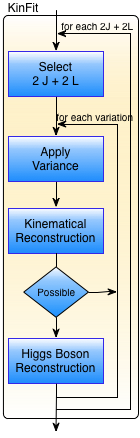
\includegraphics[scale=0.5]{images/sequential_kinfit.png}}
		\raisebox{-0.5\height}{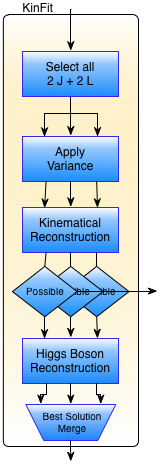
\includegraphics[scale=0.5]{images/parallel_kinfit.png}}
		\caption{Schematic representation of the \ttDilepKinFit sequential (left) and parallel (right) workflows.}
		\label{fig:SeqPipeline}
	\end{center}
\end{figure}

A shared memory parallelization using OpenMP was devised, as it is the bes approach for single shared memory systems. The parallel tasks are grouped into threads, which holds the best reconstruction to minimize the complexity of the merge by reducing through all the threads instead of tasks. The amount of tasks for each thread is balanced dynamically by the OpenMP scheduler, as the workload is irregular since the Higgs boson reconstruction execution is not always computed. Each thread has a private PRNG initialized with different seeds to avoid correlation between the numbers generated.

\begin{figure}[!htp]
	\begin{center}
		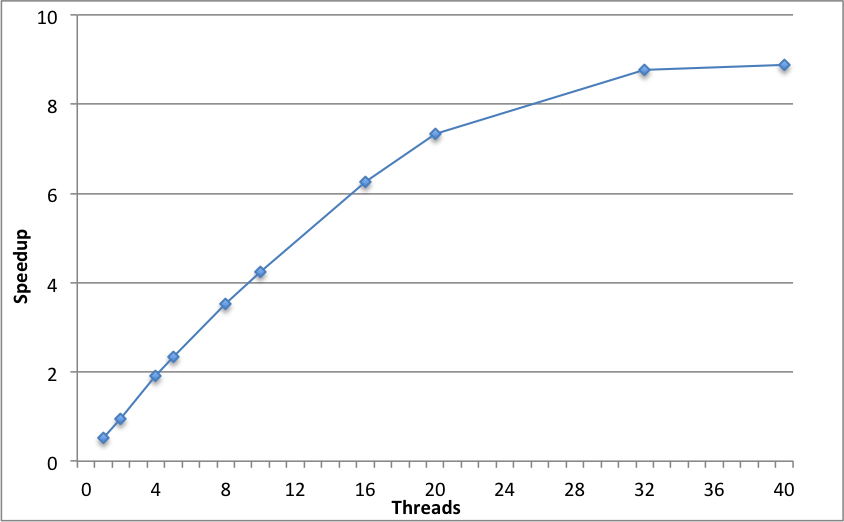
\includegraphics[scale=0.4]{charts/speedup_non_pointer_omp.png}
		\caption{Speedup for \tth parallel non-pointer version application.}
		\label{fig:non_pointer_speedup}
	\end{center}
\end{figure}

Figure \ref{fig:non_pointer_speedup} presents the speedups for various variations and threads. The purpose of the 1 thread test is to evaluate the parallelization overhead. The application has a constant scaling up to 64 variations but tends to stabilize for more variations. The best efficiency occurs when using 2 and 4 threads, where the application is almost using all resources from the cores used. The best overall performance occurs for 40 threads, but it only offers a speedup close to 16, a bit far from the theoretical limit offered by the 20 physical cores on the system. Note that there is no significant overhead due to NUMA accesses, as seen by the difference in performance from 10 to 16 threads.

% ------------- pointer version abaixo -----------------

Intel's VTune was used to search for hotspots (bottlenecks) on the parallel \tth, since this tool is best suited for profiling parallel applications while providing an easy to use GUI. A preliminary analysis revealed that the application was spending around 20\% of the time building the combination data structure for 256 variations.

An analysis of the data structure code revealed that there were inefficiencies that were affecting the performance in specific situations. Data that is read-only on the parallel section is being replicated in each element of the data structure. If the elements were to share a pointer to such data, the overhead of constructing the data structure would be reduced. However, this could lead to worse cache management, due to cache line invalidations proportional to the number of threads, resulting in added overhead, specifically in NUMA environments where the communication cost is increased. Nevertheless, this optimization was implemented and tested (addressed as \textit{pointer version}), with its speedups presented in figure \ref{fig:pointer_speedup}.

\begin{figure}[!htp]
	\begin{center}
		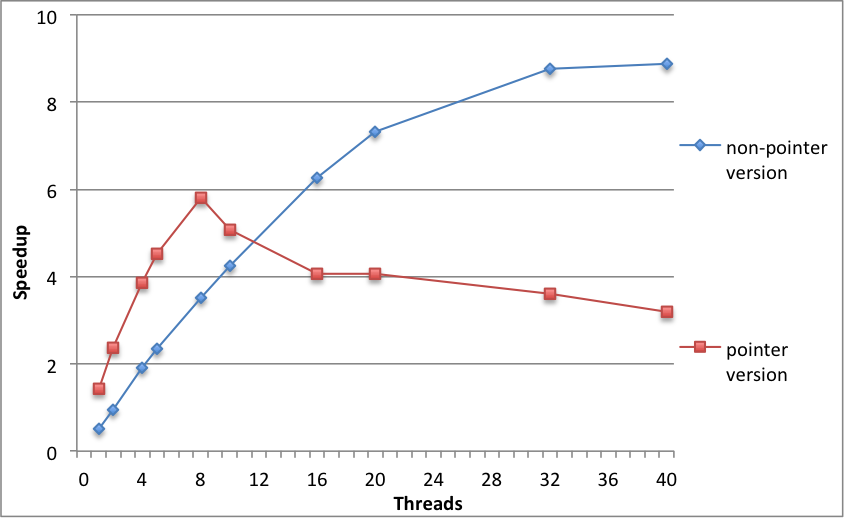
\includegraphics[scale=0.4]{charts/speedup_pointer_omp.png}
		\caption{Speedup for \tth parallel pointer version application.}
		\label{fig:pointer_speedup}
	\end{center}
\end{figure}

As predicted, the best speedup occurs when using only one CPU device, specifically for 8 threads. Even with 10 threads the performance of the application suffers due to the increase of concurrent accesses to the L3 cache on the system due to the shared data. This decrease in performance is even more noticeable when using both CPU devices, where the non-pointer version still scales while this version performance is worse than with one CPU device. However, this implementation is more efficient than the former when using only one device. Note that the superlinear speedups are due to the PRNG optimization and the reduction in the data that each thread has to process, making it more suitable to be stored in the private L2 cache of each core, therefore reducing the slower accesses to L3 cache.
